%
% jacobi.tex
%
% (c) 2021 Prof Dr Andreas Müller, OST Ostschweizer Fachhochschule
%
\documentclass[tikz]{standalone}
\usepackage{times}
\usepackage{amsmath}
\usepackage{txfonts}
\usepackage[utf8]{inputenc}
\usepackage{graphics}
\usetikzlibrary{arrows,intersections,math}
\usepackage{ifthen}
\begin{document}

\newboolean{showgrid}
\setboolean{showgrid}{false}
\def\breite{7}
\def\hoehe{4}

\begin{tikzpicture}[>=latex,thick]

\clip (-6.2,-2.5) rectangle +(12.6,4.5);

% Povray Bild
\begin{scope}[xshift=-4.2cm]
\node at (0,0) {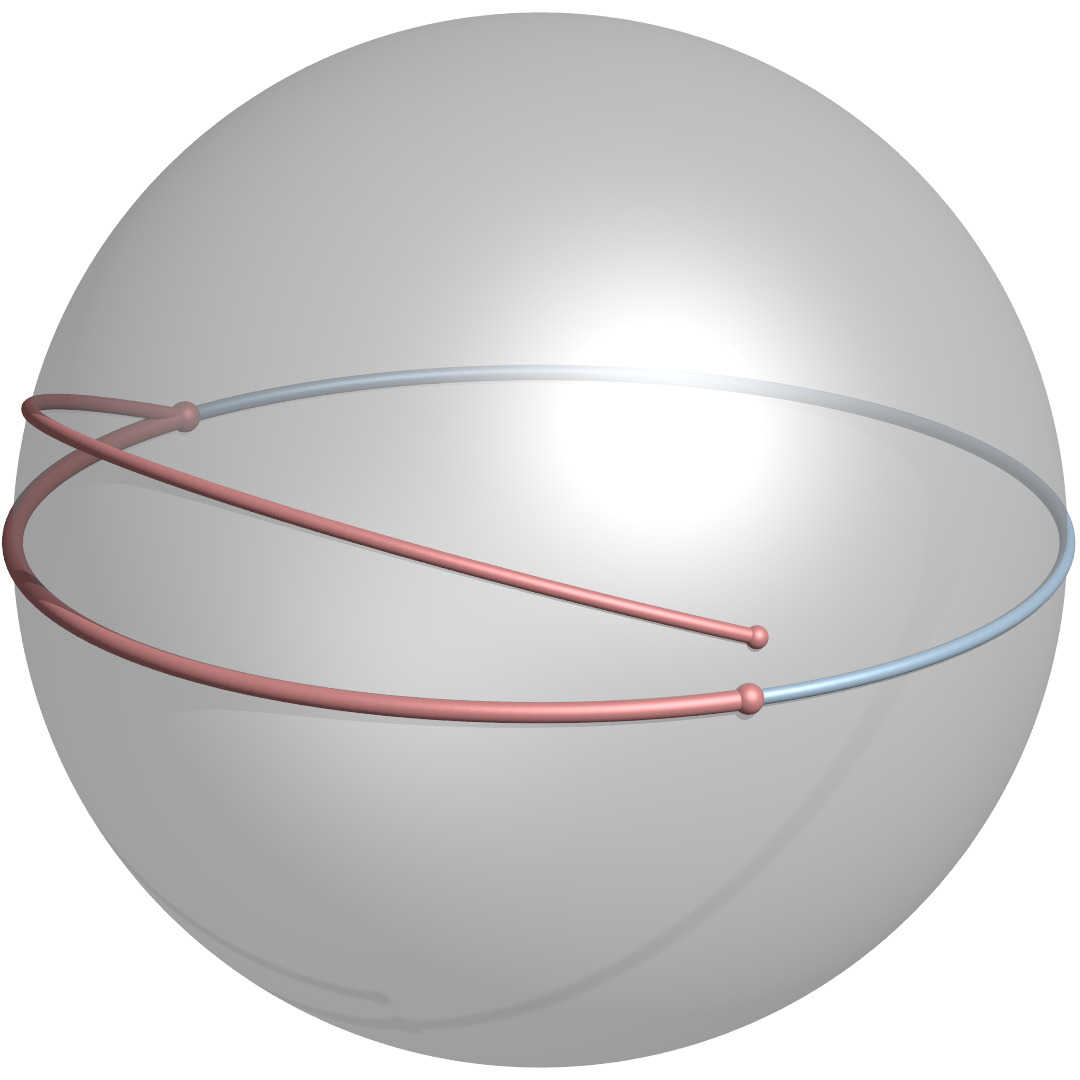
\includegraphics[width=4.00cm]{jacobi0.jpg}};
\node at (-1.3,0.7) {$x_0$};
\node at (0.8,-0.8) {$x_1$};
\node at (0,-2) [below] {a)\strut};
\end{scope}

\begin{scope}
\node at (0,0) {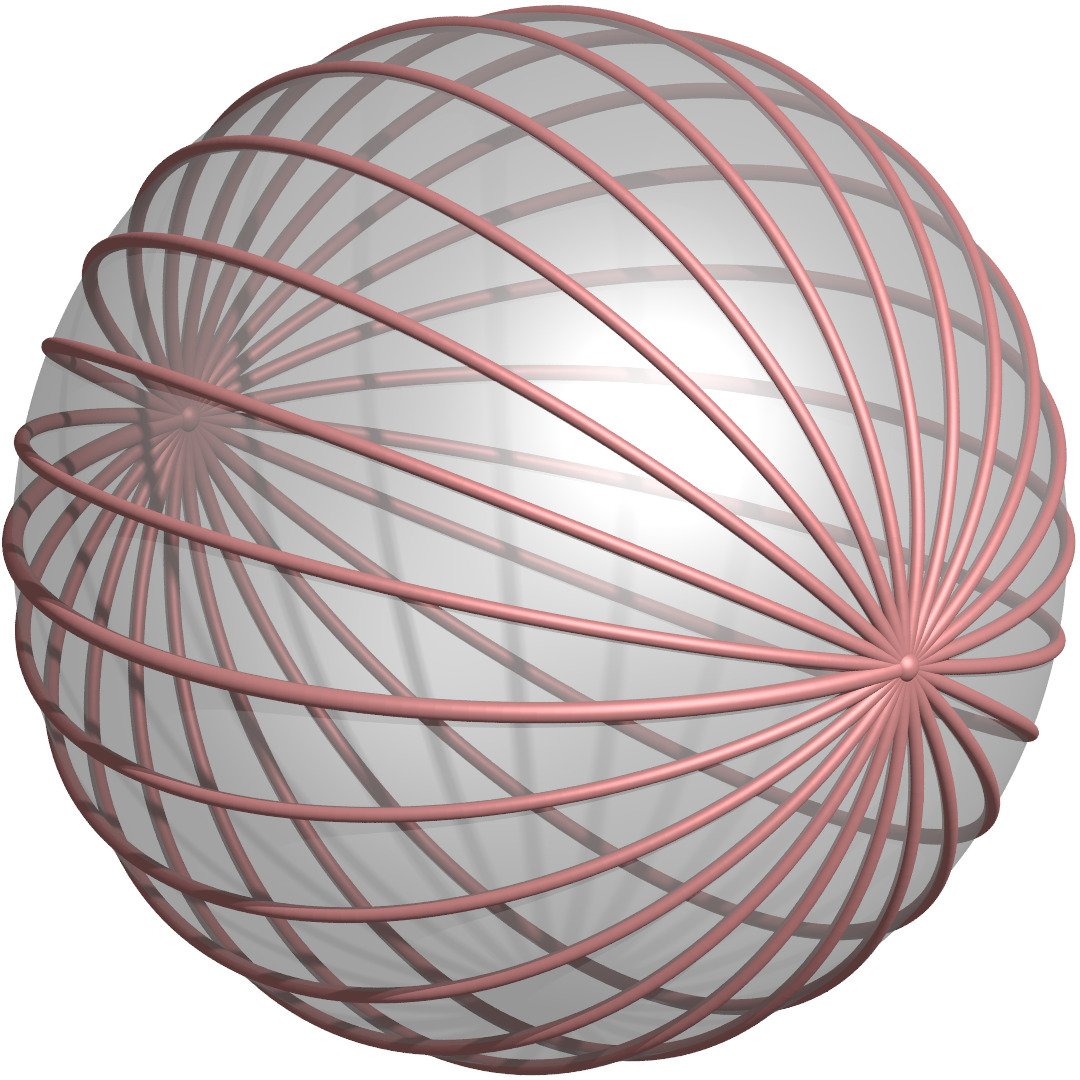
\includegraphics[width=4.00cm]{jacobi1.jpg}};
\node at (-1.2,0.2) {$x_0$};
\node at (1.4,-0.8) {$x_1$};
\node at (0,-2) [below] {b)\strut};
\end{scope}

\begin{scope}[xshift=4.2cm]
\node at (0,0) {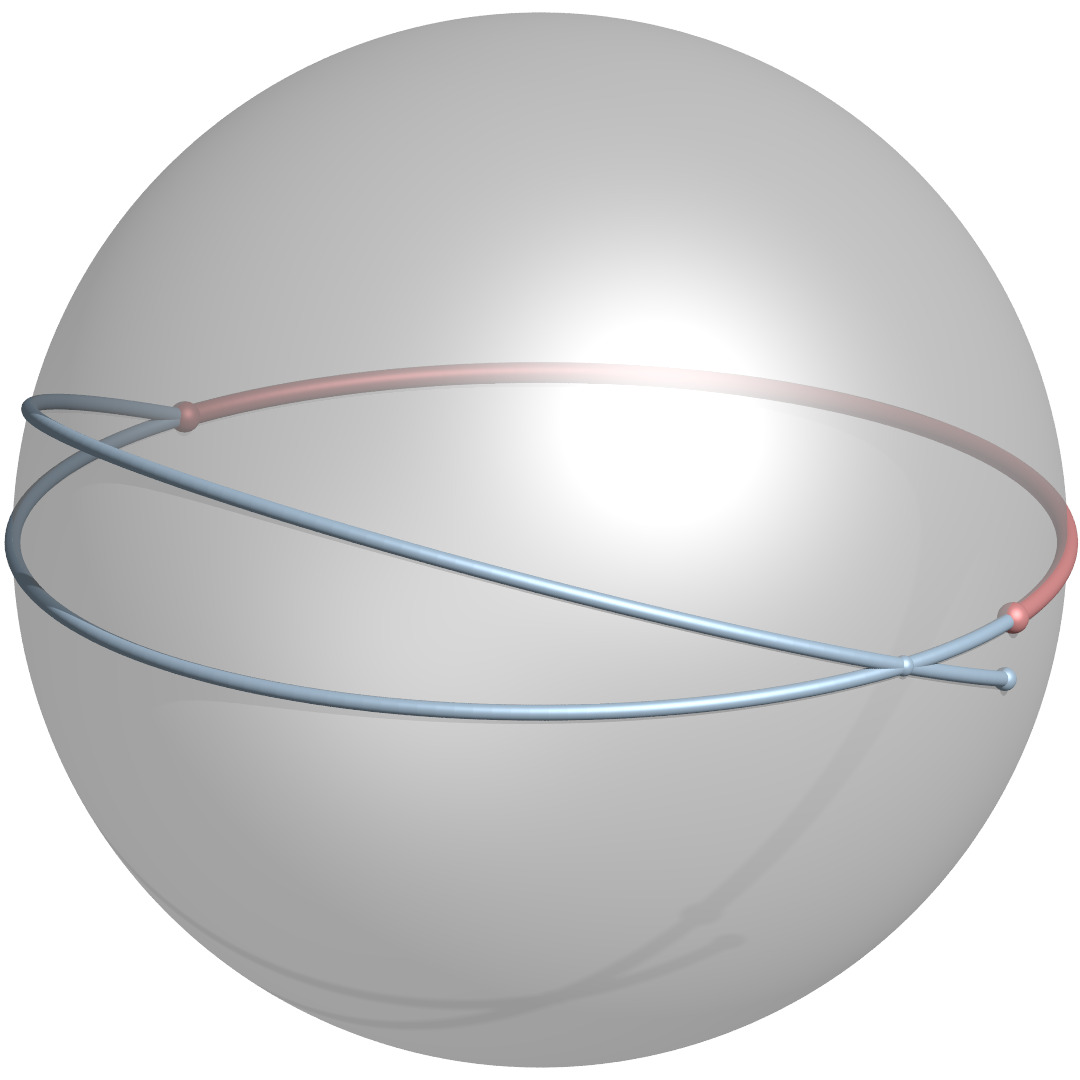
\includegraphics[width=4.00cm]{jacobi2.jpg}};
\node at (-1.3,0.7) {$x_0$};
\node at (1.3,-0.3) {$x_*$};
\node at (1.95,-0.5) {$x_1$};
\node at (0,-2) [below] {c)\strut};
\end{scope}

% Gitter
\ifthenelse{\boolean{showgrid}}{
\draw[step=0.1,line width=0.1pt] (-\breite,-\hoehe) grid (\breite, \hoehe);
\draw[step=0.5,line width=0.4pt] (-\breite,-\hoehe) grid (\breite, \hoehe);
\draw                            (-\breite,-\hoehe) grid (\breite, \hoehe);
\fill (0,0) circle[radius=0.05];
}{}

\end{tikzpicture}

\end{document}

